\documentclass[10pt,a4paper]{article}

\usepackage[utf8]{inputenc}


\usepackage{algpseudocode}
\usepackage{algorithmicx}
\usepackage{amsfonts}
\usepackage{amsmath}
\usepackage{amssymb}
\usepackage[spanish]{babel}
\usepackage[style=nature,intitle=true,sorting=none]{biblatex}
\usepackage{csquotes}
\usepackage{dsfont}
\usepackage{enumitem}
\usepackage{fancyhdr}
\usepackage{geometry}
\usepackage{graphicx}
\usepackage[hidelinks]{hyperref}
\usepackage{ifthen}
\usepackage[utf8]{inputenc}
\usepackage{multicol}
\usepackage{titling}
\usepackage{xcolor}
\usepackage{wrapfig}


\title{Organización del Computador II}
\author{Gianfranco Zamboni}

%%%% CONFIGURACIONES %%%%

%% La coma de los reales es un punto
\decimalpoint

%%% Tamaño de pagina
%\geometry{
%	includeheadfoot,
%	left=2.54cm,
%	bottom=1cm,
%	top=1cm,
%	right=2.54cm
%}

%\stul{0.1cm}{0.2ex}

%% HEADER Y FOOTER
\pagestyle{fancy}

\fancyhf{}

\fancyhead[LO]{\rightmark} % \thesection\ 
\fancyhead[RO]{\small{\thetitle}}
\fancyfoot[CO]{\thepage}
\renewcommand{\headrulewidth}{0.5pt}
\renewcommand{\footrulewidth}{0.5pt}
\setlength{\headsep}{1cm}
\setlength{\headheight}{13.07225pt}

\renewcommand{\baselinestretch}{1.2}  % line spacing

%% Links en indice 
\hypersetup{
	linktoc=all,     %set to all if you want both sections and subsections linked
	linkcolor=blue,  %choose some color if you want links to stand out
}

\newcommand{\red}[1]{{\color{red}#1}}  			% Rojo, duh (?)
\begin{document}
	\maketitle
	\tableofcontents

\newpage
\section{Introducción}

La \textbf{arquitectura de computadoras} es la ciencia y arte de diseñar las interfaces hardware/software para crear un sistema computacional que posea los requerimientos funcionales, de perfomance, consumo (de energía) y de costo (económico) adecuados para realizar determinadas tareas.

\begin{wrapfigure}{r}{0.5\textwidth}
	\centering
	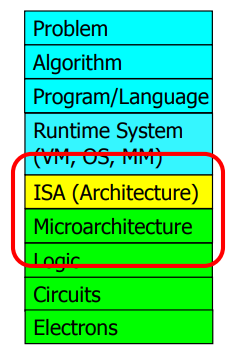
\includegraphics[width=0.25\textwidth]{imagenes/arquitectura}
	\caption{figure}{La computadora definida en niveles de abstracción}
	\label{fig:intro::arquitectura}
\end{wrapfigure}

Estas tareas son problemas que pasaron por varias transformaciones (desde su descripción en un lenguaje natural hasta convertirse en un programa) y deben ser ejecutadas por una computadora. La tarea del arquitecto consiste en diseñar el \textbf{Instruction Set Architecture} (ISA), un conjunto de instrucciones que usarán los programas compilados para decir al micropocesador que hacer. El ISA es implementado por un conjunto de estructuras de hardware conocidas como \textbf{microarquitectura}.

El ISA y la microarquitectura sientan las bases para que el diseño del procesador que conseguir el balance adecuado de los factores mencionados para llevar a cabo ciertas tareas de la manera más optima posible. Habrá casos en los que daremos prioridad a un subconjunto de ellos en detrimento de otros (por ejemplo, podriamos elegir mejorar perfomance y aumentar el costo, o quitar performance para mejorar el consumo energético).

\subsection{Componentes del ISA}
El ISA es la especificación completa de la interfaz entre los programas y el hardware que debe llevar a cabo las operaciones. Entre otras cosas, especifica:

\subsubsection{Regitros}
\begin{itemize}
	\item \textbf{Registros:} Celdas de memoria dentro del cpu que son usados para almacenar los datos necesarios para ejecutar una instrucción. Éstos son visibles al programa y se clasifican según su uso: Acumuladores, De dirección ó De Proposito General.
	\item  \textbf{Instrucciones}: Tareas que pueden ser llevadas a cabo por la computadora. Cada una de ellas está compuesta por su \textbf{opcode} (que se espera que la computadora haga) y sus \textbf{operandos} (a que datos debe hacerlo). En una ISA, podremos encontrar tres tipos de instrucciones:
	\begin{itemize}
		\item De \textbf{Operacion}: Procesan datos.
		\item De \textbf{trasnporte}: Transportan información entre la memoria, los registros y los dispositivos de entrada salida.
		\item De \textbf{control (Branching)}: Modifican la secuencia de instrucciones a ser ejecutada, es decir, permiten ejecutar instrucciones que no están almacenadas secuencialmente.
	\end{itemize}
	
	Dependiendo que valores puedan modificar las instrucciones de operación, podremos clasificar las arquitecturas en: \textbf{Arquitecturas Load/Store} (solo pueden operar en registros) o \textbf{Arquitecturas memory/memory} (se pueden modificar los valores directamente en memoria)
	\item \textbf{Tipos de datos}: Representación deben tener ciertos valores para que puedan ser interpretados por la microarquitectura.
	\item \textbf{Espacio de memoria}: La cantidad de bloques univocamente distinguibles en memoria y el tamaño de cada uno de estos bloques
	\item \textbf{Direccionamiento}: Los mecanismos usados por la computadora para saber donde están almacenados los datos. Puede ser:
	\begin{itemize}
		\item \textbf{Inmediato:} El operando está incluido en la instrucción.
		\item \textbf{Directo o absoluto:} El operando es la dirección de memoria donde se encuentra el valor a ser utilizado.
		\item \textbf{Indirecto:} El operando es una dirección de memoria donde se encuentra la dirección de memoria en la que está almacenado el valor deseado.
		\item \textbf{De desplazamiento:} La instrucción toma como operandos una dirección de memoria que se toma como \textbf{base} y un \textbf{offset}, que es un número que indica cuanto hay que desplazar la base para encontrar el valor deseado, es decir $dir = base + offset$
		\item \textbf{Indexado:} Lo mismo que el anterior, pero con el \textit{offset} guardado en un registro.
		\item \textbf{De Memoria Indirecta:} El operando es un registro en el que se encuentra guardada la dirección de memoria indirecta.
	\end{itemize}
	\item \textbf{I/O Interface}: Como comunicarse con los dispositivos de entrada/salida. Puede ser por medio de instrucciones especiales o mapeos de ciertas regiones memoria para uso de esos dispositivos.
	\item \textbf{Modos de privilegio:} Quien puede y quien no puede ejecutar ciertas instrucciones 
	\item \textbf{Manejo de expcepciones e interrupciones:} Qué debe suceder si una instrucción falla o cuando un dispositivo necesita usar el microprocesador.
	\item \textbf{Soporte de memoria virtual:} Si soporta o no el uso de \textbf{memoria virtual}, es decir, si cada programa tiene la ilusión de estar un espacio de memoria secuencial cuando en realidad el sistema operativo realiza el manejo de la memoria principal.
\end{itemize}

\subsubsection{Arquitectura de Von Neumann}\label{sec::Intro::ISA::Von_Neuman}
Como se vió en Organización del computador I, las mayoría de las ISA usadas actualmente usan el modelo de Von Neumann. Éste es un ciclo de cuatro etapas: 

\begin{enumerate}
	\item \textbf{Fecth:} Se utiliza un \textbf{program counter} para saber donde está almacenada la proxima instrucción a ser ejecutada. Y se carga desde la memoria.
	\item \textbf{Decode:} Se decodifica la instrucción fetcheada y se consiguen los operandos (literales y registros) correspondientes.
	\item \textbf{Execute:} En esta etapa se busca en memoria los datos requeridos (si es necesario) y se procesa los datos acorde a la instrucción.
	\item \textbf{Write Back:} Se almacenan los resultados obtenidos en el lugar indicado.
\end{enumerate}

\begin{figure}[h]
	\centering
	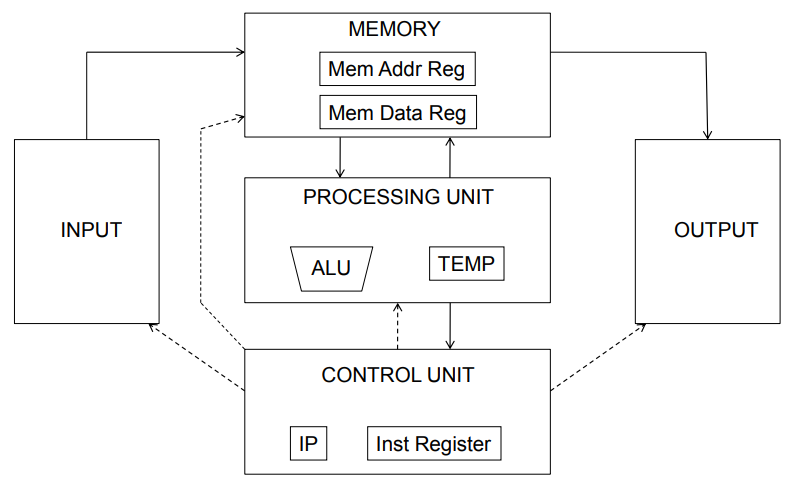
\includegraphics[width=0.4\textwidth]{imagenes/von-neuman-arquichtecture}
	\caption{Arquitectura de Von Newmman}
	\label{fig:intro:componentesIsa::vonsneumanarquichtecture}
\end{figure}
Cada instrucción es extraída de la memoria usando la dirección indicada por el \textbf{Instruction Pointer}. La unidad de control se encarga de indicar a la memoria si son necesarios otros valores para poder llevar a cabo su ejecución y luego pasa todo los datos a la unidad de procesamiento.

Si bien este es el ciclo que ``ve'' un programador, la implementación de las ISA (microarquitectura) usa estructuras de hardware más complejas que permiten acelerar la ejecución de cada fase.

\subsection{Microarquitectura}
La micoarquitectura es la implementación a nivel hardware de la ISA, es decir, es un conjunto de componentes electrónicos organizados de cierta manera para que respeten esas especificaciones. En la sección \ref{sec::Intro::ISA::Von_Neuman}, vimos como el usuario ve el ciclo de instrucciones. Desde el punto de vista de la implementación (hardware), el ciclo es realizado por unidades de procesamiento que operan sobre los datos de acuerdo a ciertas señales. 

Cada instrucción es una señal que usa el procesador de instrucciones para decidir que conjunto de componentes electrónicos deben ser activados para poder llevar a cabo la operación deseada. Especificamente, las instrucciones indican: 

\begin{itemize}
	\item \textbf{Datapath:} Que elementos deben manejar y transformar los datos (unidades de procesamiento, de almacenamiento y estructuras de hardware que permiten el flujo de datos)
	\item \textbf{Control Logic:} Que elementos de hardware determinan las señales de control que indican al datapath lo que debe hacer con los datos.
\end{itemize}

En otras palabras, la microarquitectura comprende la tecnología utilizada para construir el hardware, la organización e interconexión de la memoria, el diseño de los bloques de CPU y la implementación de distintos mecanismos de procesamiento que no son visibles para el programador. Algunas de las características encontradas en las microarquitecturas actuales son:

\begin{itemize}
	\item Pipelining
	\item Ejecución de múltiple instrucciones simultáneamente.
	\item Ejecución fuera de orden
	\item y Cachés de dato e instrucciones separadas, entre otros.
\end{itemize}

%\subsection{Medidas de Performance}
%La escala y complejidad de los sistemas de software modernos, junto con las técnicas usadas por los diseñadores de hardware para mejorar el rendimiento de los dispositivos, ha logrado hacer que el rendimiento pueda depender de varios factores.
%
%\subsubsection{Response time}
%A veces, mediremos el rendimiento de una computadora en base a su tiempo de respuesta (\textbf{response time} o \textbf{execution time}) - el tiempo entre que pasa entre que una tarea empieza y termina -. Este tiempo se mide en segundos por programa y mide el tiempo total que toma completar una tarea, incluyendo accesos a memoria, operaciones del sistema, etc.
%
%En la práctica, la computadora es compartida por varios programas y los microprocesadores deben ejecutar varias tareas simultáneamente. En estos casos, deberemos tener en cuenta que la tarea que la tarea que se está evaluando, no está siendo ejecutada todo el tiempo por lo qué habrá que distinguir el tiempo que el procesador pasa ejecutando la tarea  \textbf{CPU Time} del tiempo en el que está procesando otros programas.
%
%Entonces, el tiempo de ejecución se define de la siguiente manera:
%
%$$Response~Time = \frac{Clock~Cycles~spent~on~task}{Clock~Rate}$$
%
%Donde \textit{Clock Cycle} son la cantidad de ciclos de reloj (ticks) que se utilizaron en la tarea y \textit{Clock Rate} es el tiempo que dura cada tick del reloj.

\newpage
\section{Pipelining}
El Pipeline es una técnica que permite superponer el procesamiento de múltiples instrucciones en una ejecución. En vez de processar una instrucción completamente (realizar todas las etapas del procesamiento: Fetch, Decode, Execute, Access, Write) y luego otra,  una vez que la primera instrucción fue fetcheada y pasa a la etapa de decodificación, se comienza a fetchear la siguiente instrucción. 

Bajo condiciones ideales y con un gran número de instrucciones, la mejora en velocidad de ejecución es directamente proporcional a la cantidad de etapas en el pipe. Es decir, un pipeline de 5 etapas, es aproximadamente 5 veces más rápido que el procesamiento secuencial.  Notemos que el pipelining no modifica el tiempo que se tarda en procesar una instrucción (\textbf{latency / latencia}), sino que mejora el perfomance aumentando la cantidad de instrucciones que se procesan por unidad de tiempo (\textbf{throughput}).

\begin{figure}[h]
	\centering
	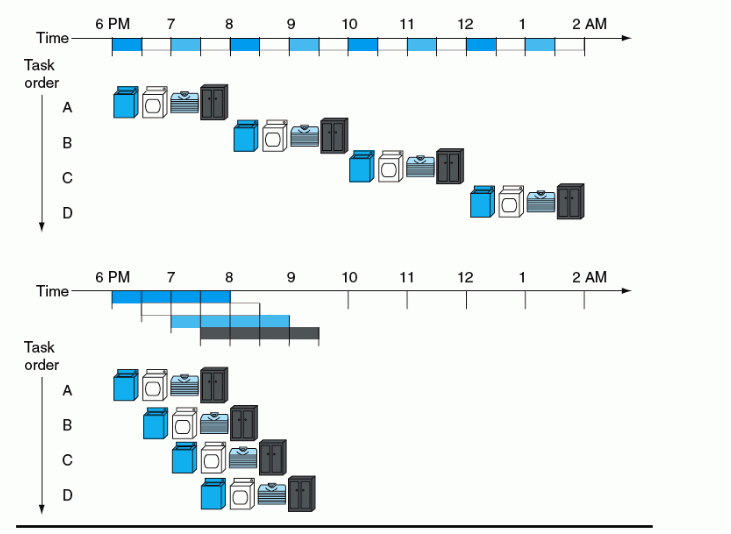
\includegraphics[width=0.5\linewidth]{imagenes/pipelining}
	\caption{Analogía de la lavandería: 4 personas tienen que lavar, secar, doblar y guardar su ropa sucia. Solo disponemos de una lavadora, una secadora, un ``doblador'' y un ropero. Si cada parte del proceso toma 30 minutos, y lo realizamos de manera secuencial, entonces completarlo para las 4 personas tomaría ocho horas, mientras que si lo hacemos con un pipeline el tiempo se reduce a tres horas y media.}
	\label{fig:pipelining}
\end{figure}

Para facilitar una implementación efectiva del pipeline, el set de instrucciones propuesto debe permitir que todas las etapas tarden el mismo tiempo en ser ejecutadas. Esto implica que hay que tener ciertas consideraciones al momento de diseñarlo:

\begin{itemize}
	\item Todas las instrucciones deben tener la misma longitud (en la arquitectura IA-32, donde las instrucciones tienen longitud variada, esto se logra descomponiendo cada instrucción en micro-operaciones de longitud fija y a estas microoperaciones se les aplica el pipelining).
	\item Todas las instrucciones deben tener la misma estructura, es decir, la cantidad de parámetros y la ubicación dentro de la instrucción que los explicita deben ser las mismas (o lo más parecidas posibles). 
	\item Los operandos deben estar alineados en memoria, esto es, las direcciones de memoria que ocupan deben ser múltiplo del tamaño de las palabras usadas para que los datos puedan ser transferidos en una única etapa del pipeline.
\end{itemize}

\subsection{Pipeline Hazards}
Hay situaciones en las que una instrucción no puede ser procesada en el siguiente ciclo de reloj. Estos eventos pueden llegar a detener el flujo del pipeline y generar una demora (\textbf{hazards}) en la ejecución del programa. A continuación veremos los tres tipos de obstáculos que se pueden dar:

\begin{itemize}
	\item \textbf{Estructurales (Structural Hazards):} El hardware no soporta la combinación de instrucciones que queremos ejecutar en el mismo ciclo de reloj. Por ejemplo, si una instrucción debe acceder a memoria mientras otra debe realizar un fetch en la misma memoria. En este caso, las dos instrucciones deben utilizar los mismos recursos y debería darsele prioridad a la primera instrucción dejando a la segunda en espera.
	\item \textbf{De datos (Data Hazards):} Hay una instrucción en el pipeline que depende de los resultados de otra (tambien en el pipeline) y debe esperar a que ésta se complete para poder terminar. Esto puede bloquear el pipe durante varios ciclos de reloj ya que se debe procesar completamente la primer instrucción. Para minimizar el impacto de este obstáculo, por lo general, se agrega extra hardware que permite conseguir el valor deseado apenas sea calculado (cuando termina la etapa de ejecución) directamente de los componentes internos para no tener que esperar a que sea guardado en memoria (esta técnica se llama \textbf{forwarding} o \textbf{bypassing}).
	\item \textbf{De control (Control or Branch Hazards):} La instrucción que se fetcheó no es la instrucción que debe ejecutarse en este ciclo de reloj. Esto sucede cuando una de las instrucciones del pipe es una instrucción condicional. En estos casos, cuando la instrucción es fetcheada, el pipeline no puede saber cual es la próxima instrucción que debe ser ejecutada ya que esto depende del resultado de la instrucción actual. Una posible solución es parar apenas se haga el fetch del condicional y esperar hasta obtener sus resultado. Otra, es realizar predicciones (\textbf{branch prediction}) y ejecutar las instrucciones con más probabilidad de ser ejecutadas. En este último caso, el pipeline procede sin demoras si la predicción fue correcta, sino debe eliminar las instrucciones procesadas y volver a comenzar desde el lugar correcto.
\end{itemize}

\newpage
\section{Branch Prediction}\label{sec::branchPrediction}

\paragraph{Branching:} Cuando se fetchea una instrucción condicional, se genera una ramificación en el código. Hay dos caminos posibles por el que puede seguir la ejecución y no tenemos seguro cual de los dos tomar.

\paragraph{Untaken Branch:} Se dice cuando el camino tomado es el que ejecuta la instrucción siguiente a la del condicional dentro del programa.

\paragraph{Taken Branch:} Cuando se ejecuta la instrucción que se encuentra en la dirección del salto de la instrucción condicional. \\


En la sección anterior se presentó la técnica de pipelining y los posibles problemas que se pueden llegar a tener cuando se usa. Uno de estos eran los problemas de control que bloqueaban el pipe cuando una de las instrucciones fetcheadas era de control. Hay diversos tipos de predicción que intentan disminuir el impacto de este problema, algunas de ellas son:

\subsection{Predicciones estáticas}
\begin{itemize}
	\item \textbf{Assume Branch Not Taken:}  Se fetchea la siguiente instrucción secuencial del programa. Si el salto no se realiza, entonces la ejecución del pipe continúa sin problemas. Si el salto se realiza, entonces se deberán descartar las instrucciones fetcheadas y decodificadas hasta el momento para poder retomar en el lugar correspondiente.
	\item \textbf{Assume Branch Taken}: Análogo al anterior, pero esta vez, se fetchea la instrucción en la dirección de memoria apuntada por el salto.
	\item \textbf{Predict by Opcode}: Se asume que el salto va a ser tomado o no dependiendo de la instrucción a ser ejecutada.
\end{itemize}

Este tipo de predicciones funcionan bien para piplines simples. Sin embargo, la penalidad de descartar instrucciones y el tiempo que se tarda en restaurar el sistema aumenta acorde a la complejidad del mismo. Las predicciones dinámicas intentan disminuir este problema manteniendo estadísticas de uso y modificando la decisiones tomadas a medida que se realiza la ejecución.

\subsection{Predicciones dinámicas}

\begin{itemize}
	\item\textbf{Branch Prediction Buffer}: Se mantiene una tabla indexada por la dirección de memoria de la instrucción del salto y 2 bits que indican si los últimos dos saltos hacia esa instrucción fueron tomados o no.
	
	\begin{figure}[h]
		\centering
		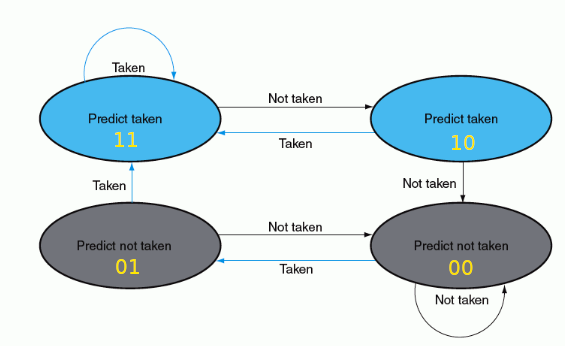
\includegraphics[width=0.7\linewidth]{imagenes/2bit-buffer-prediction}
		\caption{Maquinas de estados de predicción para un buffer de 2 bits}
		\label{fig:2bit-buffer-prediction}
	\end{figure}

	Las primeras implementaciones de esta técnica hacían uso de un único bit que se remplazaba cada vez que la predicción fallaba. En ciertos casos, la eficiencia de este método no era satisfactoria llegando a fallar completamente en otros(por ejemplo, si los saltos termina formando una secuencia intercalada de Taken y Not taken).
	
	\item \textbf{Branch Target Buffer (BTB)}: Es una caché en la que se almacena en cada entrada la dirección de la instrucción de control y la dirección de la instrucción que fue ejecutada despues de resolver el branching.
	
	Cuando se fetchea una instrucción de control, se accede a esta caché usando el valor del program counter.
	\begin{itemize}
		\item Si el valor no está en el buffer, entonces se asume \textit{taken}.
		\begin{itemize}
			\item Si el resultado es \textit{Non-Taken} se acepta el delay en el pipeline y no se almacena nada en el BTB.
			\item Si el resultado es \textit{taken}, se ingresa el valor al BTB.
		\end{itemize}
		\item Si el valor se encuentra en el BTB, se aplica el campo de dirección de target almacenado.
		\begin{itemize}
			\item si el resultado es \textit{taken}, no hay penalidad, y no se guarda en el BTB ningún nuevo valor ya que el que está almacenado es el que nos sirve.
			\item Si el resultado es \textit{Non-taken}, guarda el nuevo valor en el BTB, luego de la penalidad correspondiente en el pipeline. 
		\end{itemize}
	\end{itemize}
\end{itemize}

\newpage
\section{Instruction Level Paralelism}
Hoy en dia la mayoría de los procesadores son superscalares, es decir, explotan la ejecución paralela de instrucciones para mejorar el rendimiento. Este modelo se desvía radicalmente del de ejecución secuencial, sin embargo, por razones de compatibilidad, se debe mantener/simular ciertos aspectos del mismo.

Este tipo de procesadores analizan los binarios secuenciales de los programas y lo paralelizan eliminando secuencialidad innecesaria. Por esta razón, los programas binarios deben ser vistos más como una especificación de lo que debe hacerse y no como lo que realmente sucede.

Más precisamente, un procesador superescalar implementa:

\begin{enumerate}
	\item Estrategias de fetch que permiten fetchear múltiples instrucciones mediante la predicción de resultados y saltos.
	\item Métodos para determinar dependencias de registros y mecanismos para comunicar esos valores cuando sea necesario durante la ejecución.
	\item Métodos para iniciar, o resolver, múltiples instrucciones en paralelo.
	\item Recursos para la ejecución en paralelo de varias instrucciones, incluyendo multiples unidades funcionales de pipelines y jerarquías de memorias capaces de atender simultáneamente múltiples referencias a memoria.
	\item Métodos para manejar datos a través de instrucciones de lectura/escritura e interfaces de memoria que tengán en cuenta el comportamiento dinámico (y muchas veces impredecibles) de las jerarquías diseñadas.
	\item Métodos para actualizar los estados del proceso en el orden correcto (para mantener la apariencia de la ejecución en orden secuencial).
\end{enumerate}

\subsection{Dependencias de instrucciones}\label{sec:instructionLevelParalelism:dependenciaDeInstrucciones}
Por lo general, se interpreta el binario de un programa como un conjunto de bloques compuestos de instrucciones contiguas. Una vez que un bloque es fetcheado, se sabe que todas sus instrucciones van a ser ejecutadas eventualmente. Cuando esto suceda, diremos que el bloque es iniciado en una \textbf{ventana de ejecución}.

Una vez que las instrucciones entran en esta ventana, son ejecutadas en paralelo teniendo en cuenta sus depencencias. Éstas, pueden ser de control o datos. Las de control son generadas por condicionales y pueden ser resueltas/optimizadas con predicciones (Seccion \ref{sec::branchPrediction}). 

Las \textbf{dependencias de datos} se da entre instrucciones que referencian el mismo espacio de memoria. En estos casos, si las instrucciones no se ejecutan en el orden correcto, puede haber errores en las operaciones. Pueden ser Verdaderas o Artificales.
\begin{itemize}
	\item \textbf{Dependencias verdaderas:} Cuando una instrucción debe leer un valor que todavía no fue generado por una instrucción previa (\textbf{Read after write hazard}).
	\item \textbf{Dependecias artificiales:} Resultan de instrucciones que deben escribir un nuevo valor en una posición de memoria pero debe esperar a que las instrucciones previas utilizen el valor actual (\textbf{Write after Read hazzard}) o cuando varias instrucciones deben escribir la misma posición de memoria (\textbf{Write after Write hazzard}).
	
	Estas dependencias son producidas por código no optimizado, por escasez de registros disponibles, por el deseo de economizar el uso de la memoría principal o por ciclos donde una instrucción puede colisionar consigo misma.
	
\end{itemize}


\subsection{Fetching and Decode}
En los procesadores superescalares, una caché de instrucciones es usada para reducir la latencia y el ancho de banda del fetching. Esta caché está organizada en bloques o lineas que contienen varias instrucciones consecutivas y almacena el tipo de cada una de ellas (si es de control, de operación, de lectura de memoria, etc). 

El program counter se utiliza para determinar la posición de una instrucción en la caché.

Si se produjo un hit, se fetchea el bloque de instrucciones y luego se le suma, al program counter, el tamaño del mismo. Si hay un miss, el caché debe pedir la instrucción buscada en memoria.

Una vez conseguido el bloque de instrucciones, se identifican el tipo de cada instrucción. Si alguna es de control, entonces se realizan las predicciones necesarias mediante alguno de los métodos nombrados en la sección \ref{sec::branchPrediction}. Luego, las instrucciones son decodificadas en \textbf{tuplas de ejecución} que contienen la operación a ser ejecutada, las identidad de los elementos donde se encuentran los parámetros de entrada y donde deben guardase los resultados. 

En el programa estático, las instrucciones utilizan los registros \textbf{lógicos} (los de la arquitectura). Por esta razón, cuando son decodificadas, cada uno de ellos es mapeado (o renombrado) a un registro físico y las dependencias artificiales son resueltas indicando a las instrucciones involucradas que usen distintos registros físicos (es decir, se mapean dos o mas régistros físicos al mismo registro lógico).

Este mapeo se guarda en una tabla que asocia cada entrada a una instrucción y permite identificar el registro lógico que le corresponde. De esta forma, cuando sea necesario actualizar el estado visible de la arquitectura, la instrucción leerá su resultado del registro físico adecuado.


Una vez que todas las instrucciones asociadas a un registro físico son completadas (modifican el estado visbile), el registro es liberado para que pueda ser usado por otro bloque de instrucciones.

\subsection{Ejecución de instrucciones}
\subsubsection{Interrupciones}
Existen dos tipos de interrupciones:
\begin{itemize}
	\item \textbf{Excepciones} (o trampas), que se genera cuando se produce un error durante la ejecución o el fetching de ciertas instrucciones. Por ejemplo, opcodes ilegales,s errores numéricos o page faults.
	\item \textbf{Interrupciones externas}: Son causadas por instrucciones específicas y dispositivos externos qué están ejecutando algún proceso. Por ejemplo las interrupciones generadas por los dispositivos de entrada/salida (mouse, teclados, pantallas), timers, etc
\end{itemize}

Cuando ocurre una interrupción, el software o el hardware (o una combinación de ambos) guardan el estado del proceso interrumpido. Este estado consiste, generalmente, del program counter, los registros y la memoria. Si el estado guardado es consistente con la arquitectura secuencial del modelo, entonces diremos que la interrupción es \textbf{precisa}. Para ser más especificos, se debe cumplir que:
\begin{enumerate}
	\item Todas las instrucciones previas a la indicada por el program counter, deben haber sido ejecutadas y deben haber modificado el estado del proceso correctamente.
	\item Ninguna de las instrucciones siguientes a la indicada por el program counter debe haber ejecutadas ni deben haber modificado el estado del proceso.
	\item Si la interrupción es causada por una excepción en una instrucción del programa, entonces el program counter guardado debe apuntar a la instrucción interrumpida.
\end{enumerate}

Si el estado guardado es inconsistente con el modelo de arquitectura secuencial y no satisface estas condiciones, entonces la interrupción es \textbf{imprecisa}. 

Hay varias formas de evitar las interrupciones imprecisas:

\subsubsection{In-Order Instruction Completion}
Las instrucciones modifican el estado del proceso solo cuando se sabe que todas las instrucciones previas están libres de excepciones. Para asegurar esto, se utiliza un registro llamado ``result shift register'' que contiene una tabla de $n$  entradas ($n$ la longitud del pipeline más largo). Una instrucción que toma $i$ ciclos de reloj reserva la $i$-ésima entrada de la tabla y en cada ciclo se la desplaza una posición hacia abajo.
\begin{figure}[h]
	\centering
	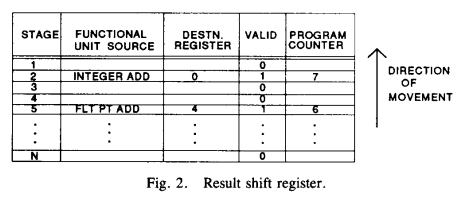
\includegraphics[width=0.5\linewidth]{imagenes/shift-register}
	\caption{Result Shift Register}
	\label{fig:shiftregister}
\end{figure}

Si la $i$-esima entrada contiene información valida, entonces la instrucción se pausa hasta el próximo ciclo de reloj y se rechequea la información de la misma.

Para evitar que una instrucción más corta se complete antes que otra de mayor longitud (cuando este es el orden deseado) se rellenan con información invalida todas las entradas anteriores que no fueron reservadas. De esta forma, la nueva instrucción es pausada hasta el próximo ciclo de reloj.

\subsubsection{Reorder-Buffer}
La principal desventaja del método anterior, es que instrucciones rápidas serán retenidas a pesar de no tener dependencias.

Para evitar esto, se permite que las instrucciones terminen en cualquier orden pero se les asigna un tag que indican el orden en el que deben modificar el estado de la computadora. Cuando son completadas, se almacena en la entrada indicada (por el tag) del buffer.

\begin{figure}[h]
	\centering
	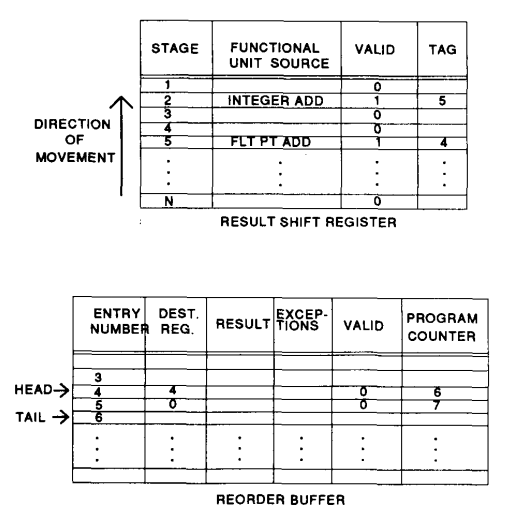
\includegraphics[width=0.5\textwidth]{imagenes/reorder-buffer}
	\caption{Reorder buffer}
	\label{fig:reorder-buffer}
\end{figure}

El buffer contiene un puntero a la entrada que corresponde a la próxima instrucción a ser ejecutada. Cuando dicha entrada contenga información valida, se  chequea si hubo excepciones. Sí no las hubo, se modifican los registros/memoria necesarios y se mueve el puntero a la próxima entrada. Sino, se emite la excepción y se invalidan todas las entradas posteriores.

En algunos casos, la dependencia entre instrucciones requiere el uso de valores que todavía no fueron escritos en los registros. Para conseguirlos es necesario acceder al buffer de reordenamiento, lo que agrega latencia y complejidad a la ejecución.

\paragraph{History Buffer:} Una solución posible es dejar que las instrucciones modifiquen los registros cuando son completadas, pero que se guarden los valores previos en un buffer que permita recuperar estos datos en el caso de una excepción.

En este caso, si ocurre una excepción, se debe recorrer el history buffer para poder recuperar un estado preciso.

\paragraph{Future File:} Otra solución es mantener dos arhicvos de registros. Uno que se actualice en el orden especificado por el programa (\textbf{Architectural File}). Y otro que se actualiza apenas se completa una instrucción (\textbf{Future File}).

Si ocurre una excepción simplemente se debe mostar el Arquitecture File para conseguir un estado preciso. Sin embargo, hay que copiarlo al future file para restaurar el estado del sistema.

\paragraph{Checkpointing:} Cuando se predice el resultado de una instruccion de control, se guarda el estado del future file (\textbf{checkpoint}). Si cuando se ejecuta la instrucción, la predicción resulta ser errónea, entonces solo hay que copiar la información del checkpoint en el future file para recuperar el estado del sistema y comenzar de nuevo en la instrucción correcta.  

\subsubsection{Out of Order Execution (Tomasulo)}
El algoritmo de Tomasulo, crea un scheduling dinamico que permite ejecutar instrucciones fuera de orden y habilita el uso de múltiples unidades de ejecución.

\paragraph{Register Renaming:} Para eliminar los WAR y WAW hazards, se utiliza una tabla llamada \textbf{Register Alias Table} que asocia un tag con cada operando de una operación.

\paragraph{Register Station (RS):} Una vez realizado el renombre se le asigna, a la instrucción un RS. Un RS es un subsistema de hardware compuesto de bancos de registros internos que se encarga de mantener las instrucciones en espera hasta que esté lista para ser ejecutada.

Un RS chequea constantemente por la disponibilidad de los operandos de la instrucción. Para cada operando cuyo valor no esté disponible, el RS, guarda el \textit{tag} que se le asignó en el paso anterior.

Cada vez que una unidad de ejecución pone disponible un operando, este transmite el \textbf{tag} asociado al operando junto con su valor a todas las RS.

Cuando una instrucción tiene todos sus operandos, el RS espera a que la unidad funcional correspondiente esté libre y luego despacha la instrucción hacia la misma.

\paragraph{Common Data Bus}: Es un datapath que cruza la salidad de las unidades funcionales y atraviesa las RS, los Floating Point Buffers, los Floating Points Registers y el Floating Point Operations Stack.

\newpage
\paragraph{Pseudocodigo}:
Cada Registro contiene un tag que indica el último escritor en el registro.

\begin{algorithmic}
\If{RS tiene discursos disponibles antes del renaming}
	\State{Se inserta en la RS la instrucción y los opernados renombrados (valor fuente / tag)}
	\State{Se renombra si y solo si la RS tiene recursos disponibles.}
	\Else
		\State{stall}
\EndIf
\While{esté en la RS, cada instrucción debe}
\State{Mirar el tráfico por el \textbf{Common Data Bus (CDB)} en busca de \textbf{tags} que corespondan a sus Operandos fuente.}
\State{Cuando se detecta un \textbf{tag}, se graba el valor de la fuente y se mantiene en RS.}
\State{Cuando ambos operandos están disponibles, la instrucciónn se marca \textbf{Ready} para ser despachada}
\If{Unidad Funcional disponible}
\State{Se depscacha la instrucción a esa unidad funcional}
\EndIf
\If{Finalizada la ejecución de la instrucción}
\State{La unidad funcional pone el valor correspondiente al \textbf{tag} en el \textbf{CBD} (\textbf{tag broadcast})}
\If{El archivo de registros está conectado al CDB}
\If{tag del Archivo de Registro $==$ tag broadcast}
\State{Registro = valor broadcast}
\State{bit de validez = '1'}
\State{Recupera \textbf{tag} renombrado}
\State{No queda copia válida del tag en el sistema}
\EndIf
\EndIf
\EndIf
\EndWhile
\end{algorithmic}
	\nocite{*}
\bibliographystyle{plain}
\bibliography{bibliography}

\end{document}

